% Options for packages loaded elsewhere
\PassOptionsToPackage{unicode}{hyperref}
\PassOptionsToPackage{hyphens}{url}
%
\documentclass[
]{article}
\usepackage{amsmath,amssymb}
\usepackage{iftex}
\ifPDFTeX
  \usepackage[T1]{fontenc}
  \usepackage[utf8]{inputenc}
  \usepackage{textcomp} % provide euro and other symbols
\else % if luatex or xetex
  \usepackage{unicode-math} % this also loads fontspec
  \defaultfontfeatures{Scale=MatchLowercase}
  \defaultfontfeatures[\rmfamily]{Ligatures=TeX,Scale=1}
\fi
\usepackage{lmodern}
\ifPDFTeX\else
  % xetex/luatex font selection
\fi
% Use upquote if available, for straight quotes in verbatim environments
\IfFileExists{upquote.sty}{\usepackage{upquote}}{}
\IfFileExists{microtype.sty}{% use microtype if available
  \usepackage[]{microtype}
  \UseMicrotypeSet[protrusion]{basicmath} % disable protrusion for tt fonts
}{}
\makeatletter
\@ifundefined{KOMAClassName}{% if non-KOMA class
  \IfFileExists{parskip.sty}{%
    \usepackage{parskip}
  }{% else
    \setlength{\parindent}{0pt}
    \setlength{\parskip}{6pt plus 2pt minus 1pt}}
}{% if KOMA class
  \KOMAoptions{parskip=half}}
\makeatother
\usepackage{xcolor}
\usepackage[margin=1in]{geometry}
\usepackage{graphicx}
\makeatletter
\def\maxwidth{\ifdim\Gin@nat@width>\linewidth\linewidth\else\Gin@nat@width\fi}
\def\maxheight{\ifdim\Gin@nat@height>\textheight\textheight\else\Gin@nat@height\fi}
\makeatother
% Scale images if necessary, so that they will not overflow the page
% margins by default, and it is still possible to overwrite the defaults
% using explicit options in \includegraphics[width, height, ...]{}
\setkeys{Gin}{width=\maxwidth,height=\maxheight,keepaspectratio}
% Set default figure placement to htbp
\makeatletter
\def\fps@figure{htbp}
\makeatother
\setlength{\emergencystretch}{3em} % prevent overfull lines
\providecommand{\tightlist}{%
  \setlength{\itemsep}{0pt}\setlength{\parskip}{0pt}}
\setcounter{secnumdepth}{-\maxdimen} % remove section numbering
\ifLuaTeX
  \usepackage{selnolig}  % disable illegal ligatures
\fi
\IfFileExists{bookmark.sty}{\usepackage{bookmark}}{\usepackage{hyperref}}
\IfFileExists{xurl.sty}{\usepackage{xurl}}{} % add URL line breaks if available
\urlstyle{same}
\hypersetup{
  hidelinks,
  pdfcreator={LaTeX via pandoc}}

\author{}
\date{}

\begin{document}

\hypertarget{notes-iwatsuki-1992-stentor-coeruleus-shows-positive-photokinesis}{%
\section{\texorpdfstring{Notes: Iwatsuki (1992) --- \emph{Stentor
coeruleus} Shows Positive
Photokinesis}{Notes: Iwatsuki (1992) --- Stentor coeruleus Shows Positive Photokinesis}}\label{notes-iwatsuki-1992-stentor-coeruleus-shows-positive-photokinesis}}

Source: Iwatsuki, K. (1992). \emph{Stentor coeruleus} shows positive
photokinesis. \emph{Photochemistry and Photobiology}, 55(3), 469--471.
(PDF:
\href{references/Iwatsuki-1992-Stentor-coeruleus-positive-photokinesis.pdf}{\texttt{references/Iwatsuki-1992-Stentor-coeruleus-positive-photokinesis.pdf}})

\hypertarget{key-findings}{%
\subsection{Key findings}\label{key-findings}}

\begin{itemize}
\tightlist
\item
  \emph{S. coeruleus} shows \textbf{positive photokinesis}: swims faster
  in light, slower in dark. Mean velocity \textasciitilde0.6 mm/s at 100
  lx, up to \textasciitilde1.0 mm/s at 50000 lx (white light).
\item
  Velocity increases roughly \textbf{linearly with log(fluence rate)}
  --- a Weber--Fechner-type relationship, not linear in raw light
  intensity.
\item
  Photokinesis has its own action spectrum, distinct from the
  photophobic-response/ phototaxis action spectrum (peak 610 nm). This
  implies \textbf{at least two separate photoreceptor systems} in the
  cell.
\item
  \emph{S. coeruleus} is reported as the first protozoan shown to
  exhibit all three photoresponse types: photophobic response,
  phototaxis, and photokinesis.
\end{itemize}

\hypertarget{figure-3}{%
\subsection{Figure 3}\label{figure-3}}

\begin{figure}
\centering
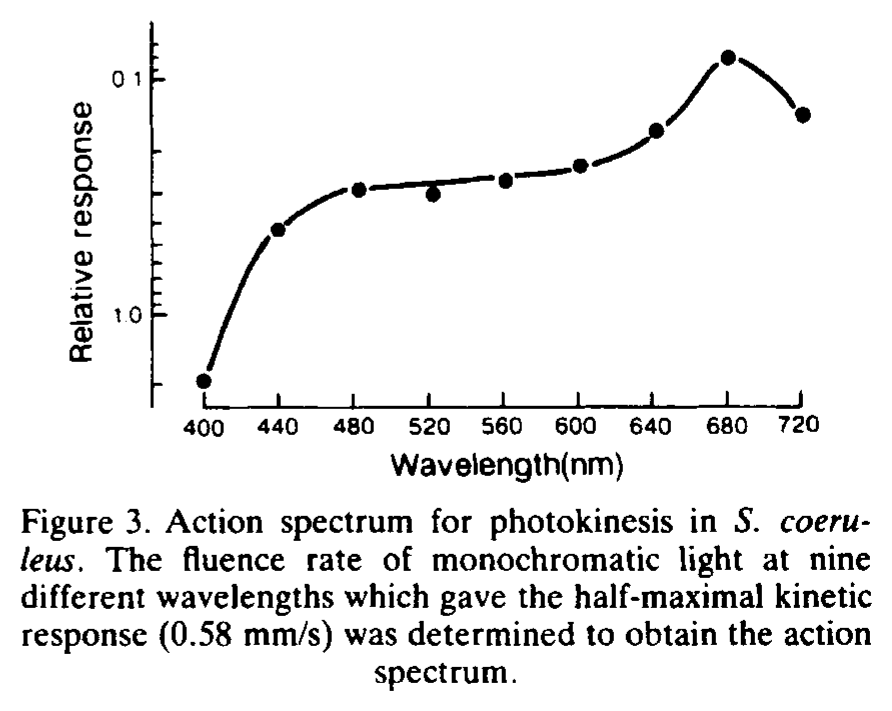
\includegraphics{references/iwatsuki-1992-figure3-action-spectrum.png}
\caption{Figure 3. Action spectrum for photokinesis in S. coeruleus.}
\end{figure}

\begin{quote}
\textbf{Figure 3. Action spectrum for photokinesis in \emph{S.
coeruleus}.} The fluence rate of monochromatic light at nine different
wavelengths which gave the half-maximal kinetic response (0.58 mm/s) was
determined to obtain the action spectrum.
\end{quote}

\hypertarget{how-figure-3-action-spectrum-was-built}{%
\subsection{How Figure 3 (action spectrum) was
built}\label{how-figure-3-action-spectrum-was-built}}

For each of 9 wavelengths (400--720 nm), the authors measured a full
fluence-rate vs. velocity dose-response curve (like the 680 nm / 440 nm
examples in Fig. 2a --- velocity rises \textasciitilde linearly with log
fluence rate). From each curve they read off the \textbf{fluence rate
required to reach a fixed criterion velocity: 0.58 mm/s} (the paper
calls this the ``half-maximal kinetic response,'' but see the ``Why 0.58
mm/s'' section below --- the paper does not describe how this specific
number was derived, and it's likely just a common target velocity within
the overlapping range of all 9 curves rather than a computed
dark-floor/light-ceiling midpoint). This lets 9 whole dose-response
curves collapse into 9 single comparable numbers (essentially an
EC50-per-wavelength), which is what's plotted as the action spectrum.

\hypertarget{reading-the-y-axis-logarithmic-and-inverted}{%
\subsubsection{Reading the y-axis: logarithmic AND
inverted}\label{reading-the-y-axis-logarithmic-and-inverted}}

\begin{itemize}
\tightlist
\item
  Y-axis label: ``Relative response.'' Y-axis units are actually the
  \textbf{fluence rate (W/m\^{}2)} needed to hit 0.58 mm/s --- same
  scale as the x-axis of Fig. 2a (log, \textasciitilde0.1--1.0+
  W/m\^{}2).
\item
  The axis is drawn \textbf{inverted} (small numbers near the top, large
  numbers near the bottom). This is a standard action-spectrum
  convention: the biologically meaningful quantity is \emph{sensitivity}
  = 1/fluence needed, not the fluence itself. Rather than plot the
  reciprocal, the axis is just flipped so ``higher on the page'' =
  ``less light was needed'' = ``more sensitive'' --- producing a
  normal-looking peaked curve even though the raw printed numbers are
  fluence rates, not sensitivity units.
\end{itemize}

\hypertarget{specific-values-discussed}{%
\subsubsection{Specific values
discussed}\label{specific-values-discussed}}

\begin{itemize}
\tightlist
\item
  \textbf{680 nm to \textasciitilde0.08 W/m\^{}2} needed to reach 0.58
  mm/s (near the top of the plot --- most sensitive point tested).
\item
  \textbf{400 nm to \textasciitilde1.1 W/m\^{}2} needed to reach 0.58
  mm/s (near the bottom --- least sensitive point tested).
\item
  Ratio \textasciitilde= \textbf{14x} --- Stentor needs roughly 14 times
  less red (680 nm) light than blue (400 nm) light to produce the same
  swimming-speed increase. This is a genuine, strong action-spectrum
  peak at 680 nm, not just a mild bias.
\item
  Curve shape across the spectrum: steep rise from 400--440 nm, a
  plateau through \textasciitilde440--600 nm, then a second climb to the
  true peak at 680 nm, followed by a drop at 720 nm.
\end{itemize}

\hypertarget{why-0.58-mms-specifically}{%
\subsection{Why 0.58 mm/s
specifically}\label{why-0.58-mms-specifically}}

\textbf{Correction / uncertainty flag:} initial notes here speculated
that 0.58 mm/s was the midpoint between a measured ``dark floor''
velocity and a measured ``saturating ceiling'' velocity. That is
\emph{not} stated anywhere in the paper's Materials \& Methods and is
likely wrong, for two reasons:

\begin{enumerate}
\def\labelenumi{\arabic{enumi}.}
\tightlist
\item
  \textbf{A true zero-light data point isn't measurable with their
  setup.} The same light source that provides the photokinetic stimulus
  also provides the dark-field illumination the ``Bug-tracker'' camera
  needs to see/track the cell at all (``To generate dark-field
  illumination and to stimulate the organisms, white light\ldots{}
  was\ldots{} projected\ldots{}''). There's no separate viewing-light
  channel, so they can't record a cell swimming in literal darkness.
\item
  \textbf{No plateau is described.} Both Fig. 1a (white light,
  100--50000 lx) and Fig. 2a (monochromatic, \textasciitilde0.1--2
  W/m\^{}2) are described as ``increased almost linearly with a
  logarithmic increase'' across the \emph{entire} tested range --- no
  floor/ceiling saturation is mentioned, so there's no natural min/max
  to average.
\end{enumerate}

\textbf{More likely explanation:} 0.58 mm/s is a fixed criterion
velocity chosen because it falls \emph{within the overlapping,
actually-measured range} of all nine wavelength-specific
fluence-response curves --- i.e., a common target every curve crosses
somewhere in its tested data, so a fluence-rate value can be read off
(interpolated, not extrapolated) for each of the 9 wavelengths. This is
the standard practical reason for picking one criterion response when
collapsing several dose-response curves into a single action spectrum;
it does not require or imply any dark/saturating-max calibration
measurement.

\end{document}
